
\subsection{Calculate References}
\label{sec:ui_proc_calc_references}

This task allows the computation of reference trajectories from associated tracks with assigned unique target numbers (see \nameref{sec:ui_associate_tr}). \\

Currently the following sensor data can be incorporated into reference track estimation.

\begin{itemize}
    \item System Tracks
    \item ADS-B \\
\end{itemize}

It is possible to exclude target reports from the estimation based on various criteria. 
The used reconstructor then integrates locations, velocities and any associated uncertainties of 
added target reports, in order to generate reference positions with estimated locations, velocities and uncertainties. \\

After reference computation the generated reference trajectories for each target will be added to the database 
as a new data source. \\

The task's dialog will show as follows. \\

\begin{figure}[H]
    \center
      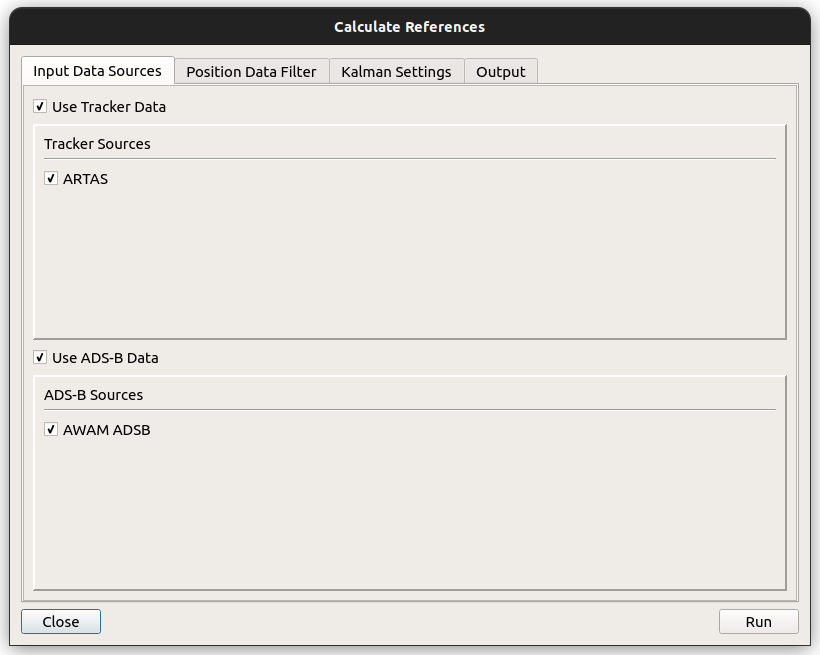
\includegraphics[width=9cm]{figures/ui_task_references_dialog.png}
    \caption{Calculate References Task - Configuration Dialog}
\end{figure}

It consists of several configuration tabs.

\begin{itemize}
    \item \textbf{Input Data Sources}: Configuration of data sources to use for reference computation.
    \item \textbf{Position Data Filter}: Filtering options for excluding certain target reports from reference computation.
    \item \textbf{Kalman Settings}: Configuration of the Kalman reconstructor.
    \item \textbf{Output}: Configuration of the generated data source. \\
\end{itemize}

These configuration tabs will be described in more detail below.

\subsubsection{Input Data Sources}

\begin{figure}[H]
    \center
      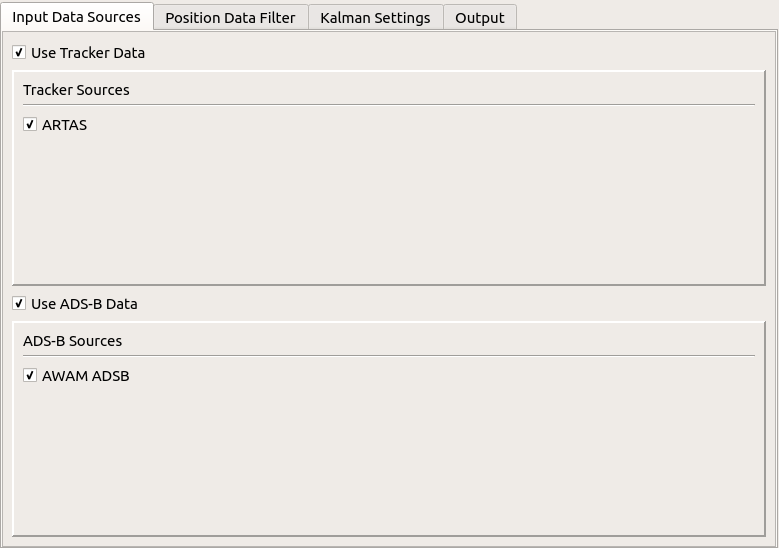
\includegraphics[width=9cm]{figures/ui_task_references_tab_inputds.png}
    \caption{Calculate References Task - Input Data Sources Tab}
\end{figure}

Here the data sources which are incorporated into reference track estimation can be configured.
There exists a checkbox for each possible DSType and then a nested list of checkboxes for individual data sources. \\

\textbf{Note}: At least one data source has to be selected in order to run reference computation.

\subsubsection{Position Data Filter}

\begin{figure}[H]
    \center
      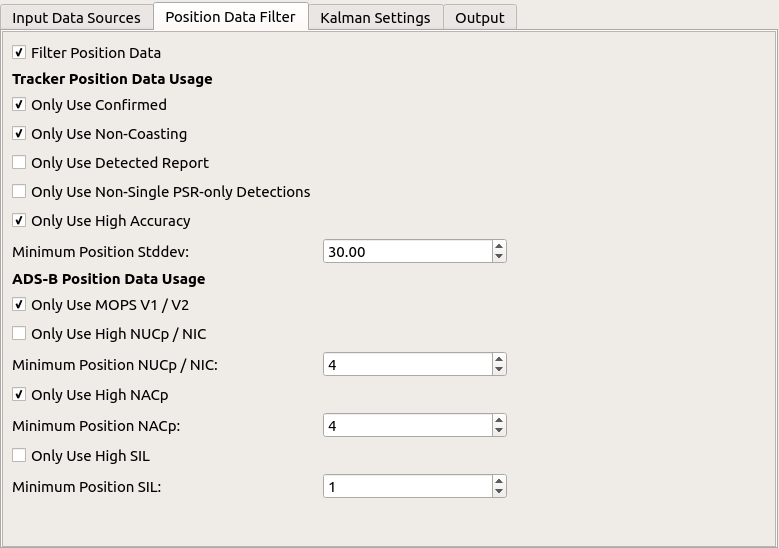
\includegraphics[width=9cm]{figures/ui_task_references_tab_filter.png}
    \caption{Calculate References Task - Position Data Filter Tab}
\end{figure}

Here various filters can be enabled in order to remove certain target reports from reference computation. 
The following tables describe the existing options.

\begin{table}[H]
    \center
    \begin{tabularx}{\textwidth}{ | l | l | X |}
        \hline
        \textbf{Parameter} & \textbf{Default} & \textbf{Description} \\ \hline
        Filter Position Data & enabled & Enables/disables filtering of position data \\ \hline
    \end{tabularx}
\end{table}

\textbf{Note}: All other options will be ignored if this option is disabled. \\

\textit{Tracker Position Data Usage}:
\begin{table}[H]
    \center
    \begin{tabularx}{\textwidth}{ | l | l | l | X |}
        \hline
        \textbf{Parameter} & \textbf{Default} & \textbf{Unit} & \textbf{Description} \\ \hline
        Only Use Confirmed & enabled & & TODO \\ \hline
        Only Use Non-Coasting & enabled & & TODO \\ \hline
        Only Use Detected Report & disabled & & TODO \\ \hline
        Only Use Non-Single PSR-only Detections & disabled & & TODO \\ \hline
        Only Use High Accuracy & enabled & & TODO \\ \hline
        Minimum Position Stddev & 30 & m & TODO \\ \hline
    \end{tabularx}
\end{table}

\textit{ADS-B Position Data Usage}:
\begin{table}[H]
    \center
    \begin{tabularx}{\textwidth}{ | l | l | X |}
        \hline
        \textbf{Parameter} & \textbf{Default} & \textbf{Description} \\ \hline
        Only Use MOPS V1 / V2 & enabled & TODO \\ \hline
        Only Use High NUCp / NIC & disabled & TODO \\ \hline
        Minimum Position NUCp / NIC & 4 & TODO \\ \hline
        Only Use High NACp & enabled & TODO \\ \hline
        Minimum Position NACp & 4 & TODO \\ \hline
        Only Use High SIL & disabled & TODO \\ \hline
        Minimum Position SIL & 1 & TODO \\ \hline
    \end{tabularx}
\end{table}

\subsubsection*{Kalman Settings}

\begin{figure}[H]
    \center
      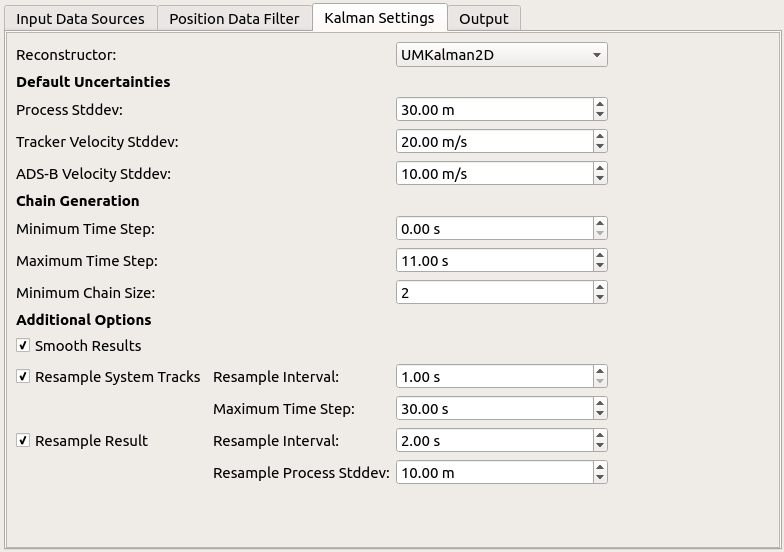
\includegraphics[width=9cm]{figures/ui_task_references_tab_kalman.png}
    \caption{Calculate References Task - Kalman Settings Tab}
\end{figure}

Here the used reference trajectory reconstructor can be chosen and configured.
The following tables describe the existing options.

\begin{table}[H]
    \center
    \begin{tabularx}{\textwidth}{ | l | l | X |}
        \hline
        \textbf{Parameter} & \textbf{Default} & \textbf{Description} \\ \hline
        Reconstructor & UMKalman2D & Reconstructor type used for reference computation \\ \hline
    \end{tabularx}
\end{table}

The currently implemented reconstructors are based on the well-known Kalman filter and its various variants.
Currently the following 'flavours' are implemented. \\

\begin{itemize}
    \item \textbf{Uniform Motion Kalman (UMKalman2D)}: 
        Classic Kalman filter assuming a constant velocity between consecutive measurements
    \item \textbf{Accelerated Motion Kalman (AMKalman2D)}: 
        Unscented Kalman filter assuming constant acceleration between consecutive measurements \\
\end{itemize}

\textit{Default Uncertainties}: Parameters related to the uncertainties used in the Kalman filter, in addition to those provided 
by the input data.
\begin{table}[H]
    \center
    \begin{tabularx}{\textwidth}{ | l | l | l | X |}
        \hline
        \textbf{Parameter} & \textbf{Default} & \textbf{Unit} & \textbf{Description} \\ \hline
        %Measurement Stddev & 30 & m & Default standard deviation for added measurements \\ \hline
        %Measurement Stddev (high) & 1000 & m & Default high standard deviation for added measurements, 
        %    used if important data is not provided by the data base (e.g. velocity) \\ \hline
        Process Stddev & 30 & m & Default standard deviation of the modelled Kalman process \\ \hline
        Tracker Velocity Stddev & 50 & m & Default standard deviation for tracker velocities, 
            used if not provided by the data \\ \hline
        %Tracker Acceleration Stddev & 50 & m & Default standard deviation for tracker accelerations,
        %    used if not provided by the data \\ \hline
        ADS-B Velocity Stddev & 50 & m & Default standard deviation for ADS-B velocities, 
            used if not provided by the data \\ \hline
        %ADS-B Acceleration Stddev & 50 & m & Default standard deviation for ADS-B accelerations, 
        %    used if not provided by the data \\ \hline
    \end{tabularx}
\end{table}

\textbf{Note}: If no position accuracy is provided by the data for a specific target report, a standard value of 30 meters is
automatically assumed. This is not the optimal case though, and it should be prevented by setting a suitable filter 
in the \textit{Position Data Filter} tab. Also note that if an important value such as velocity is
not provided by the data, a value of zero with a very high standard deviation of 1000 meters is automatically assumed. \\

\textit{Chain Generation}: Parameters related to criteria causing the reconstructor to reinitialize the Kalman filter, 
resulting in the reference trajectory of a track being split into multiple sub-chains.
\begin{table}[H]
    \center
    \begin{tabularx}{\textwidth}{ | l | l | l | X |}
        \hline
        \textbf{Parameter} & \textbf{Default} & \textbf{Unit} & \textbf{Description} \\ \hline
        Minimum Time Step & 0 & s & Minimum time difference between consecutive measurements (measurements obtaining a 
            lower time difference to their predecessor will be skipped) \\ \hline
        Maximum Time Step & 11 & s & Maximum time difference between consecutive measurements (measurements obtaining a 
            higher time difference to their predecessor will cause the Kalman filter to reset, 
            resulting in a new sub-chain) \\ \hline
        Minimum Chain Size & 2 & & Minimum number of created reference positions in a sub-chain, in order to add the chain 
            to the final result \\ \hline
    \end{tabularx}
\end{table}

\textit{Additional Options}:
\begin{table}[H]
    \center
    \begin{tabularx}{\textwidth}{ | X | l | l | X |}
        \hline
        \textbf{Parameter} & \textbf{Default} & \textbf{Unit} & \textbf{Description} \\ \hline
        Smooth Results & enabled & & Smooth the results of the Kalman filter using a Rauch–Tung–Striebel smoother \\ \hline
        Resample System Tracks & enabled & & Resample input system tracks using cubic spline interpolation \\ \hline
        Resample System Tracks - Resample Interval & 1 & s & Time interval at which system tracks are resampled \\ \hline
        Resample System Tracks - Maximum Time Step & 30 & s & Maximum time difference between consecutive tracker 
            reports in order to resample the segment \\ \hline
        Resample Result & enabled & & Resample the generated reference trajectories by interpolating the final Kalman states
            at a fixed rate \\ \hline
        Resample Result - Resample Interval & 2 & s & Time interval at which the result trajectories are resampled \\ \hline
        Resample Result - Resample Process Stddev & 10 & m & Standard deviation of the Kalman process when interpolating the 
            Kalman states during result resampling \\ \hline
    \end{tabularx}
\end{table}

Resampling of system tracks can be enabled in order to obtain similar sample rates for tracker and ADS-B
data, which reduces a sensor-specific bias of the Kalman filter. Cubic B-splines are used to interpolate the tracker target
reports in a relaxed way. In case a spline segment deviates too strongly from its interval, a linear interpolation is 
chosen instead. \\

Result resampling can be enabled in order to obtain reference trajectories with a homogeneous sample rate. 
It is carried out by interpolating the Kalman states at fixed time-steps. The accuracy of the resulting samples
follows the Kalman accuracies more closely when interpolating near the endpoints of a segment, and it will decrease
in the middle of a segment. The amount of decrease of accuracy will depend on the time duration of the segment and the used 
process standard deviation (parameter \textit{Resample Process Stddev}).

\subsubsection{Output}

\begin{figure}[H]
    \center
      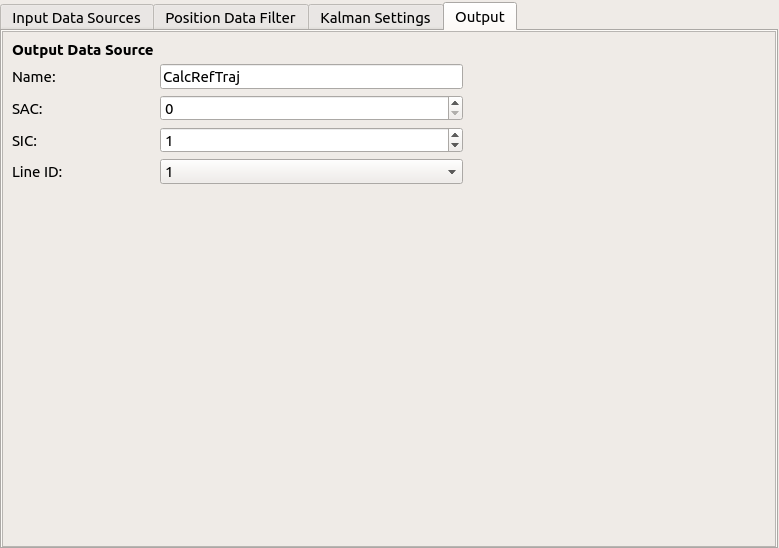
\includegraphics[width=9cm]{figures/ui_task_references_tab_info.png}
    \caption{Calculate References Task - Output Tab}
\end{figure}

Here the data source created by reference computation can be configured. 
Reference data will be stored to the database as part of this data source.
The following options are available. \\

\textit{Output Data Source}:
\begin{table}[H]
    \center
    \begin{tabularx}{\textwidth}{ | l | l | X |}
        \hline
        \textbf{Parameter} & \textbf{Default} & \textbf{Description} \\ \hline
        Name & CalcRefTraj & Name of the created data source \\ \hline
        SAC & 0 & SAC of the created data source \\ \hline
        SIC & 1 & SIC of the created data source \\ \hline
        Line ID & 1 & Line ID under which the created data is stored \\ \hline
    \end{tabularx}
\end{table}

\textbf{Note} that an already existing reference data source is just updated by running the 
reference computation again. This way it is possible to store several reference trajectories to 
different line IDs for the sake of comparison.

\subsubsection{Running The Task}

If configured correctly, the task can be started by clicking the \textit{Run} button.
The current configuration can always be stored without running the task by clicking the \textit{Close} button. 
This can be useful when changing the configuration for tuning features such as TODO (link to Show Intermediate Results). \\

When the task is started, the following progress dialog is shown to the user.

\begin{figure}[H]
    \center
      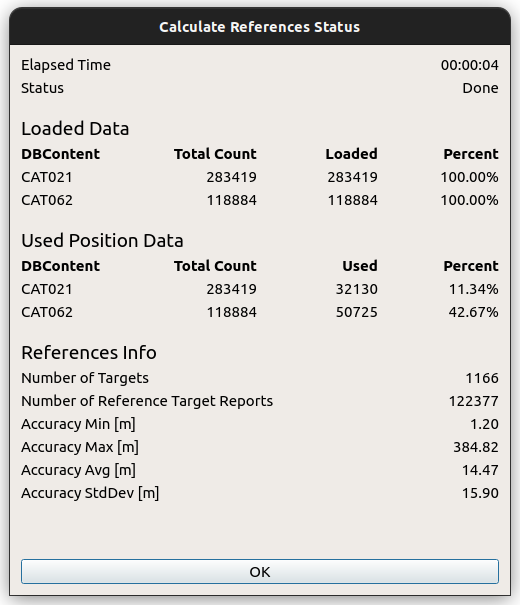
\includegraphics[width=9cm]{figures/ui_task_references_dialog_result.png}
    \caption{Calculate References Task - Calculate References Status Dialog}
\end{figure}

First the elapsed time and the current status of the reconstruction process are shown.
Then a few sections give more inside into what happened in the various stages of the process, 
which are described in more detail below.

\paragraph{Loaded Data} This section gives insight into to what degree data has been loaded from
the database. It shows total and currently loaded data counts, and loading percentage, broken down into
individual DSTypes.

\paragraph{Used Position Data} This section gives insight into to what degree loaded data has been
included in the reconstruction process after filtering. 
It shows total data counts, and the amount of data items used for reconstruction in absolute numbers and percentages,
broken down into individual DSTypes.

\paragraph{References Info} This section displays information about the reference computation result.
It shows the number of reference trajectories created, the total number of created target reports, and 
accuracy statistics, which can be used to quantify how well the reconstructor performed.
